The controls layer is responsible for binding all modules of the Turing Board to be part of the same system. All data coming in is intercepted by this layer and forwarded to the respective modules responsible for processing the forwarded data.

\subsection{Layer Hardware}
The hardware involved in the Nvidia Jetson TX2 which is responsible for running the controls code.

\subsection{Layer Operating System}
The Layer makes use of the Linux operating system to run applications such as the control code.

\subsection{Layer Software Dependencies}
Python Dependencies
\begin{itemize}
    \item PyVESC
    \item Pyrebase
    \item Pyserial
    \item Pycrc
    \item Threading
\end{itemize}

\subsection{Jetson TX2 Subsystem}
The Jetston TX2 is the main computing power for the Turing board. It is responsible for processing all input from the remote control and computer vision. From there, it is responsible for sending the appropriate signals to the peripherals.

\begin{figure}[h!]
	\centering
 	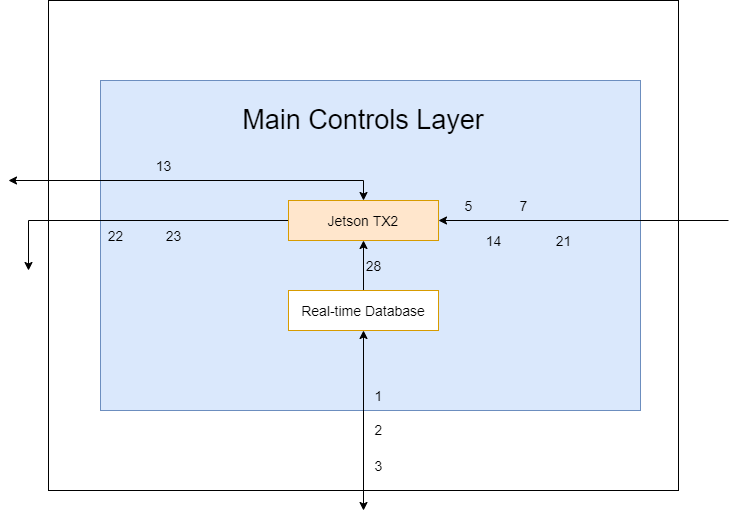
\includegraphics[width=0.60\textwidth]{images/Jetson.png}
 \caption{Jetson TX2 Subsystem in Main Controls Layer}
\end{figure}

\subsubsection{Subsystem Hardware}
The Jetson TX2 connects with the JetPack 4.6 on a host machine. 

\subsubsection{Subsystem Operating System}
The Jetson TX2 is flashed with Ubuntu 18.04 LTS.

\subsubsection{Subsystem Software Dependencies}
The install of Ubuntu 18.04 installs the following items:
\begin{itemize}
    \item cuDNN 8.2.1
    \item CUDA 10.2
    \item OpenCV4.1.1 - which will be removed later since OpenCV must be complied from source to take advantage of the CUDA cores
\end{itemize}

\subsubsection{Subsystem Programming Languages}
The Jetson TX2 uses Python as its programming language.

\subsubsection{Subsystem Data Structures}
Classes
\begin{itemize}
    \item Controls
    \begin{itemize}
        \item Responsible for running the controls code.
    \end{itemize}
    \item Serial Communication
    \begin{itemize}
        \item Establishes connection with the microcontroller.
    \end{itemize}
\end{itemize}

\subsubsection{Subsystem Data Processing}
After fetching data from the database, the Jetson TX2 will process the data first to an extent. Since data coming in will be floating point values, it first needs to be translated into value which the microcontroller can understand. So, the entire range of data from the remote control app is taken and the required data is mapped from 0-255 which is then forwarded to the microcontroller which causes the wheels to change speed. As part of the same data packet, angle data from the controls code is also sent to the microcontroller which aids in turning the turning mechanism to a specific angle with respect to the turning mechanisms origin. Any data such as weight values if someone is standing on the long board is received back in the same data format (0-255) which gets translated to weight values inside of the controls code.

\subsection{Real-Time Database Subsystem}
There are three main components of project which calls for this piece of software which must all be non-blocking in nature to ensure the entire system stays responsive.
\begin{itemize}
    \item Reading data from the microcontroller.
    \item Forwarding data to the microcontroller.
    \item Fetching data from the Firebase Real-time database.
\end{itemize}

\begin{figure}[h!]
	\centering
 	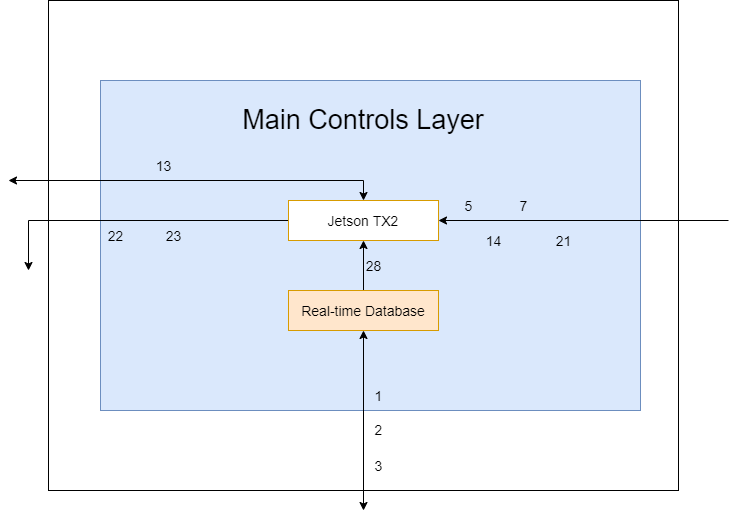
\includegraphics[width=0.60\textwidth]{images/RTD.png}
 \caption{Real-time Database Subsystem in Main Controls Layer}
\end{figure}

\subsubsection{Subsystem Hardware}
The real-time database subsystem does not consist of explicit hardware. All work is done through software to communicate information.

\subsubsection{Subsystem Operating System}
The real-time database subsystem does not make use of an underlying operating system. The layer makes use of the Linux operating system.

\subsubsection{Subsystem Software Dependencies}
Python Dependencies
\begin{itemize}
    \item PyVESC
    \item Pyrebase
    \item Pyserial
    \item Pycrc
    \item Threading
\end{itemize}

\subsubsection{Subsystem Programming Languages}
Python
\begin{itemize}
    \item Used for the main controls system.
\end{itemize}

\subsubsection{Subsystem Data Structures}
The real-time data base fetching process utilizes hashmaps to send and receive data. 

\subsubsection{Subsystem Data Processing}
As data is updated in the database, it is fetched and brought to the Jetson TX2 for processing. For more information on the process within the Jetson, see section 4.4.6.
